\documentclass[border=0pt]{standalone}
\usepackage{tikz}
\usetikzlibrary{calc}

\definecolor{bgtop}{HTML}{0E1D3F}
\definecolor{bgbot}{HTML}{050A17}
\definecolor{city}{HTML}{13244D}
\definecolor{cityfar}{HTML}{0F1C3D}
\definecolor{steel}{HTML}{A9BCD3}
\definecolor{panel}{HTML}{2B3F66}
\definecolor{bA}{HTML}{38BDF8}
\definecolor{bB}{HTML}{F5A524}
\definecolor{bC}{HTML}{34D399}
\definecolor{bD}{HTML}{E879F9}

% \beam{x0}{y0}{x1}{y1}{color}: lobe from the array at (x0,y0) toward a user at (x1,y1)
\newcommand{\beam}[5]{%
  \pgfmathsetmacro{\dx}{#3-#1}\pgfmathsetmacro{\dy}{#4-#2}%
  \pgfmathsetmacro{\ang}{atan2(\dy,\dx)}%
  \pgfmathsetmacro{\L}{sqrt(\dx*\dx+\dy*\dy)-0.62}%
  \pgfmathsetmacro{\w}{0.055*\L+0.10}%
  \begin{scope}[shift={(#1,#2)},rotate=\ang]
    \foreach \s/\o in {1.00/0.10, 0.72/0.16, 0.45/0.28, 0.20/0.55}{
      \fill[#5,opacity=\o]
        (0,0) .. controls ({0.30*\L},{1.30*\w*\s}) and ({0.82*\L},{1.15*\w*\s}) .. (\L,0)
              .. controls ({0.82*\L},{-1.15*\w*\s}) and ({0.30*\L},{-1.30*\w*\s}) .. (0,0);
    }
    % wavefronts travelling along the beam
    \foreach \t in {0.30,0.48,0.66,0.84}{
      \pgfmathsetmacro{\r}{\t*\L}\pgfmathsetmacro{\a}{atan(0.95*\w/\r)}
      \draw[#5,opacity=0.85,line width=0.9pt,line cap=round]
        ({\r*cos(-\a)},{\r*sin(-\a)}) arc[start angle=-\a,end angle=\a,radius=\r];
    }
  \end{scope}
}

% \phone{x}{y}{color}
\newcommand{\phone}[3]{%
  \begin{scope}[shift={(#1,#2)}]
    \fill[#3,opacity=0.18] (0,0) circle (0.78);
    \fill[#3,opacity=0.22] (0,0) circle (0.52);
    \fill[black!85,rounded corners=2.6pt] (-0.24,-0.44) rectangle (0.24,0.44);
    \draw[#3,line width=1.1pt,rounded corners=2.6pt] (-0.24,-0.44) rectangle (0.24,0.44);
    \fill[#3!30!black,rounded corners=1pt] (-0.185,-0.34) rectangle (0.185,0.35);
    \fill[black!85] (-0.06,0.355) rectangle (0.06,0.40);
    % signal bars on the screen
    \foreach \i/\h in {0/0.08,1/0.14,2/0.20,3/0.26}{
      \fill[#3] ({-0.12+\i*0.075},-0.20) rectangle ({-0.075+\i*0.075},{-0.20+\h});
    }
  \end{scope}
}

\begin{document}
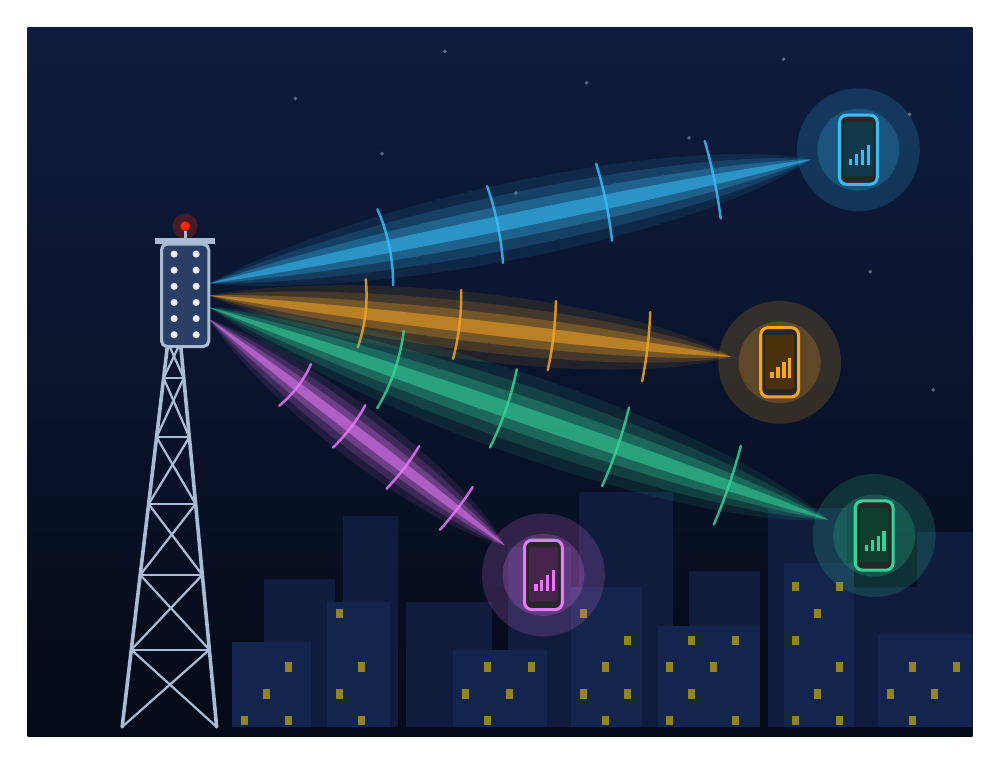
\begin{tikzpicture}
  \useasboundingbox (0,0) rectangle (12,9);
  \clip (0,0) rectangle (12,9);

  % sky
  \shade[top color=bgtop,bottom color=bgbot] (0,0) rectangle (12,9);
  \foreach \x/\y in {7.1/8.3,9.6/8.6,11.2/7.9,5.3/8.7,3.4/8.1,8.4/7.6,10.7/5.9,6.2/6.9,4.5/7.4,11.5/4.4}{
    \fill[white,opacity=0.35] (\x,\y) circle (0.025);
  }

  % far skyline
  \foreach \x/\w/\h in {3.0/0.9/2.0,4.0/0.7/2.8,4.8/1.1/1.7,6.1/0.8/2.4,7.0/1.2/3.1,8.4/0.9/2.1,9.4/1.0/2.9,10.5/0.8/1.9,11.3/0.9/2.6}{
    \fill[cityfar] (\x,0) rectangle ++(\w,\h);
  }
  % near skyline with lit windows
  \foreach \x/\w/\h in {2.6/1.0/1.2,3.8/0.8/1.7,5.4/1.2/1.1,6.9/0.9/1.9,8.0/1.3/1.4,9.6/0.9/2.2,10.8/1.3/1.3}{
    \fill[city] (\x,0) rectangle ++(\w,\h);
    \pgfmathsetmacro{\nx}{int(\w/0.28)}\pgfmathsetmacro{\ny}{int(\h/0.34)}
    \foreach \i in {1,...,\nx}{\foreach \j in {1,...,\ny}{
      \pgfmathsetmacro{\lit}{mod(\i*7+\j*13+int(\x*10),5)}
      \ifdim\lit pt<1.5pt
        \fill[yellow!70!orange,opacity=0.55] ({\x+\i*0.28-0.17},{\j*0.34-0.20}) rectangle ++(0.09,0.12);
      \fi
    }}
  }
  \fill[bgbot] (0,0) rectangle (12,0.12);

  % beams (drawn before the tower so the array sits on top)
  \beam{2.30}{5.75}{10.55}{7.45}{bA}
  \beam{2.30}{5.60}{9.55}{4.75}{bB}
  \beam{2.30}{5.45}{10.75}{2.55}{bC}
  \beam{2.30}{5.30}{6.55}{2.05}{bD}

  % base-station tower (lattice mast)
  \begin{scope}[steel,line width=1.3pt,line cap=round,line join=round]
    \draw (1.20,0.12) -- (1.78,5.00);
    \draw (2.40,0.12) -- (1.94,5.00);
    \foreach \y/\yy in {0.12/1.10,1.10/2.05,2.05/2.95,2.95/3.80,3.80/4.55,4.55/5.00}{
      \pgfmathsetmacro{\xl}{1.20+(\y-0.12)/4.88*0.58}\pgfmathsetmacro{\xr}{2.40-(\y-0.12)/4.88*0.46}
      \pgfmathsetmacro{\xll}{1.20+(\yy-0.12)/4.88*0.58}\pgfmathsetmacro{\xrr}{2.40-(\yy-0.12)/4.88*0.46}
      \draw[line width=0.8pt] (\xl,\y) -- (\xrr,\yy);
      \draw[line width=0.8pt] (\xr,\y) -- (\xll,\yy);
      \draw[line width=0.8pt] (\xll,\yy) -- (\xrr,\yy);
    }
  \end{scope}

  % antenna array panel
  \fill[panel,rounded corners=2pt,draw=steel,line width=1.1pt] (1.70,4.95) rectangle (2.30,6.25);
  \foreach \i in {0,1}{\foreach \j in {0,...,5}{
    \fill[white,opacity=0.9] ({1.86+\i*0.28},{5.10+\j*0.205}) circle (0.045);
  }}
  \fill[steel] (1.62,6.25) rectangle (2.38,6.33);
  % beacon
  \fill[red!70!orange] (2.00,6.48) circle (0.06);
  \fill[red!70!orange,opacity=0.25] (2.00,6.48) circle (0.16);
  \draw[steel,line width=1pt] (2.00,6.33) -- (2.00,6.42);

  % users
  \phone{10.55}{7.45}{bA}
  \phone{9.55}{4.75}{bB}
  \phone{10.75}{2.55}{bC}
  \phone{6.55}{2.05}{bD}
\end{tikzpicture}
\end{document}
